\chapter{Antriebsstrang}
\fancyfoot[C]{Lackner}


%% Übersicht %%%%%%%%%%%%%%%%%%%%%%%%%%%%%%%%%%%%%%%%%%%%%%%
\section{Übersicht}
Die Hauptaufgabe des Anrtiebssystems ist die Umwandlung der, von dem Akkumulator zur Verfügung gestellten, elektrischen Energie in die kinetische Antriebsenergie. Diese tritt zuerst kreisförmig am Motor auf und wird zunächst über das Direkt-Getriebe umgeformt bzw. auf die passende Drehzahl gebracht, anschließend wird die kreisförmige kinetische Energie mithilfe des Hinterrades auf die Straße übertragen und das ganze Motorrad beschleunigt. Neben dem Antrieb des Motorrades hat die Motorsteuerung noch weitere Bedeutung als Steuereinheit, diese fungiert als Bindemittel zwischen dem Human-Computer Interacting System und den elektrischen Anforderungen an das Gesamtsystem.


\subsection{Grundfunktionen des Systems}
Die geplanten Funktionen des Antriebssystems lassen sich grob in zwei Grundfunktionen einteilen:

\begin{itemize}
	\item Der Antrieb - Translation ist eine Grundfunktion eines jeden Verkehrsmittels
	\\ Durch die Umwandlung der elektrischen Energie in kinetische Energie erfährt 
	\\ das gesamte System eine Beschleunigung in Fahrtrichtung.
	\item Die Steuereinheit - Steuerung und Kommunikation mit anderen Betriebsmitteln
	\\ Realisiert durch In- und Outputs, Datenübetragung mithilfe des CAN-Buses 
\end{itemize}

Um auf die einzelnen Details des Antriebssystems besser eingehen zu können, unterscheiden wir zwischen dem Hardwareaufbau und dem Softwareaufbau des Antriebssystems.

\newpage



%% Hardwareaufbau %%%%%%%%%%%%%%%%%%%%%%%%%%%%%%%%%%%%%%%%%%%%%%%
\section{Hardwareaufbau des Antriebssystems}
Der grundsätzliche Hardwareaufbau des Antriebssystems lässt sich in zwei galvanisch getrennte Stromkreise und der mechanischen Umsetzung unterscheiden:

\begin{itemize}
	\item Mechanische Umsetzung (Kraftübertragung und Montage) 
	\\ Umfasst das Getriebe und die Befestigung aller Komponenten am Rahmen.
	\item Der Laststromkreis
	\\ Beinhaltet die Verbindung des Motorcontrollers mit dem Motor und dem Akkumulator.
	\item Der Steuerstromkreis
	\\ Beinhaltet alle elektrischen Verbindungen, welche mithilfe des 35-poligen
	\\ Niederleistungs-Steckers mit dem Motorcontroller verbunden sind.
\end{itemize}

\newpage



%% Mechanische Umsetzung %%%%%%%%%%%%%%%%%%%%%%%%%%%%%%%%%%%%%%%%%%%%%%% 
\subsection{Mechanische Umsetzung}
Die Fertigung des Getriebes und die Montage der einzelnen Betriebsmittel wurde vollständig von Tobias Schmeisser übernommen.


\newpage



%% Der Laststromkreis %%%%%%%%%%%%%%%%%%%%%%%%%%%%%%%%%
\subsection{Der Laststromkreis}
Der Laststromkreis befasst sich mit allen leistungsführenden Betriebsmitteln des Antriebssystems. ierbei unterscheiden wir zwischen zwei Grundfunktionen:

\begin{itemize}
	\item Elektrische Energieübertragung
	\\ Umfasst die elektrische Verbindung von Motor, Motorcontroller und Akkumulator. 						\\ Realisiert durch einfache Leitungen, um Leistungen übertragen zu können.
	\item Schutz aller Komponenten vor möglichen Beschädigungen (Leitungsschutzorgane)
	\\ Beinhaltet eine Schmelzsicherung zum Schutz vor Überströmen und ein 									\\ Hochleistungs-Relais, um im Fehlerfall den kreis öffnen zu können und damit  		
	\\ eine galvanische Trennung des Antriebs und der Energieversorgung gewährleisten zu können.
\end{itemize}

\begin{figure}[H]
	\begin{center}
		%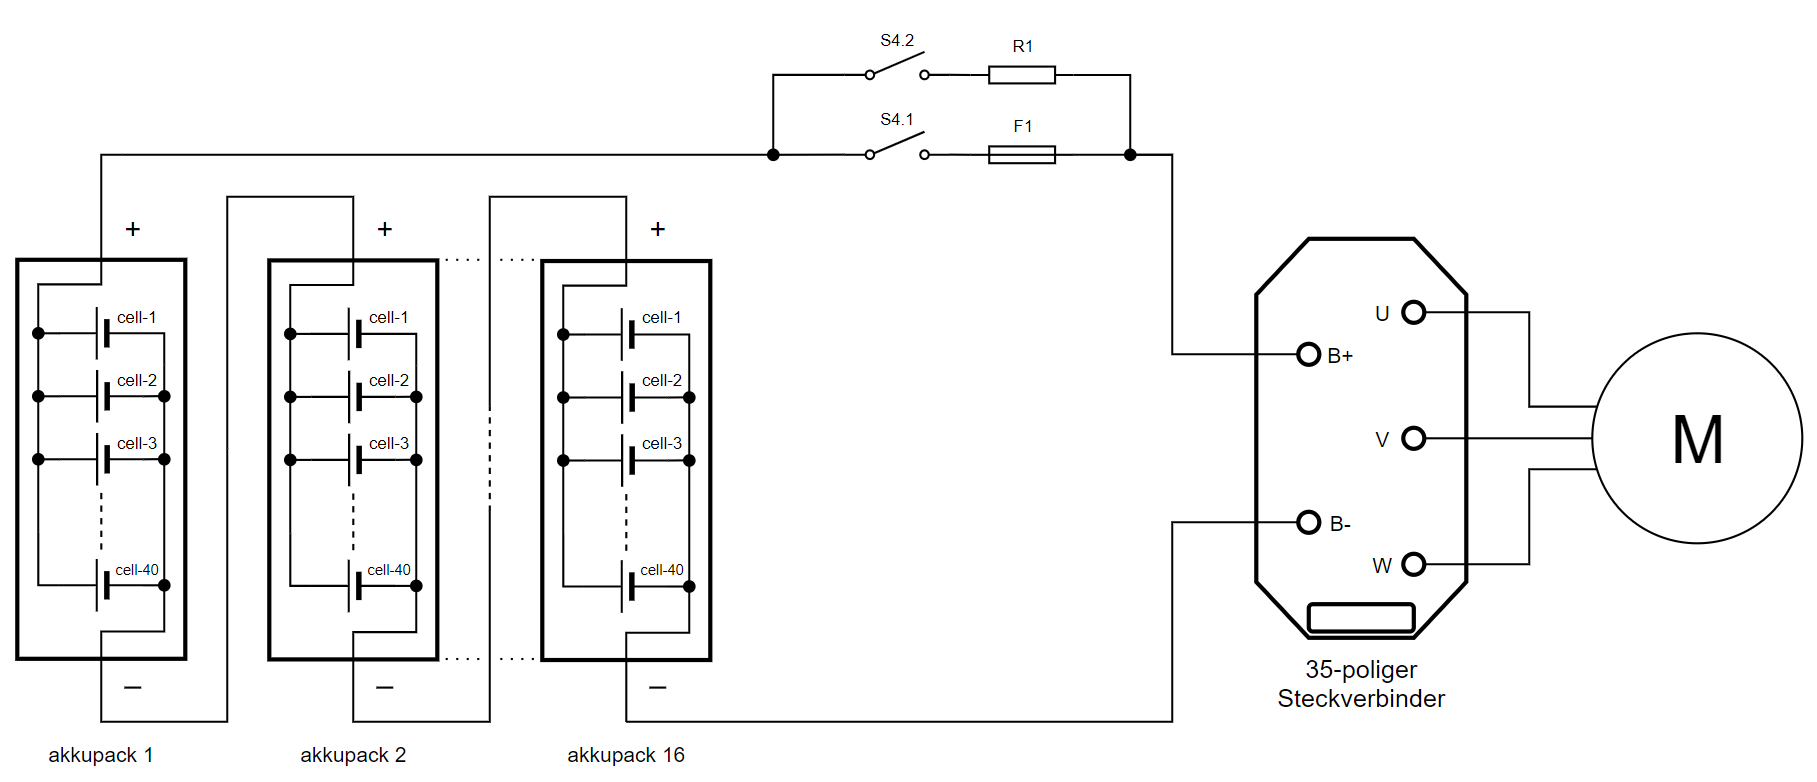
\includegraphics[scale=0.5]{figures/hcis/Antrieb_Laststromkreis.png}
		\caption{Grundaufbau des Laststromkreises}
	\end{center}
\end{figure}

\newpage



%% Elektrische Energieübertragung %%%%%%%%%%%%%%%%%%%%%%%%%%%%%%%%%
\subsubsection{Elektrische Energieübertragung}
Um die benötigte elektrische Energie übertragen zu können, müssen die Leitungen an den Leistungsverbrauch des Verbrauchers (Motor) angepasst werden. Bei einer zu hohen Stromaufnahme (Überlast) des Motors kann es zu einer übermäßigen Erwärmung der Leitungen bis hin zu dauerhaften Beschädigungen, wie durchschmorren der Isolierung oder sogar einen Leitungsbrand, führen. Um dies verhindern zu können, müssen die Leitungen an die Stromaufnahme des Motors angepasst werden. Das heißt, der zulässige Dauerstrom der Leitungen muss den maximalen Dauerstrom des Motors bzw. den maximalen Dauerstrom, welcher durch den Akkumulator zur Verfügung gestellten werden kann, übersteigen.

Berechnung:
In diesem Abschnitt befassen wir uns zunächst mit der Berechnung aller Ströme, die wir zur Auswahl der richtigen Leitungen benötigen. Bei der Auswahl von Leitungen muss man grundsätzlich den Querschnitt und die Länge der Leitung an die benötigte Stromaufnahme des Motors anpassen.

Auswahl:

Fazit:

\newpage



%% Leitungsschutzorgane %%%%%%%%%%%%%%%%%%%%%%%%%%%%%%%%%
\subsubsection{Leitungsschutzorgane}
Die Aufgabe der Leitungsschutzorgane ist es, bei unerwarteten Überströmen oder in einem Fehlerfall den Laststromkreis zu öffnen und damit den Motor bzw. Motorcontroller und den Akkumulator galvanisch zu trennen, um mögliche Beschädigungen an den Komponenten oder an den Leitungen verhindern zu können. Da jedoch ungewünschte Fehlauslösungen zum sofortigen Stillstand des Motorrades führen und eventuell sogar benötigte Wartungen (Wechsel der durchgebrannten Schmelzsicherung) nach sich ziehen, müssen diese Leitungsschutzorgane sehr sorgfältig ausgewählt werden. Eine Überdimensionierung ist ebenso unerwünscht, denn dies hat nicht nur höhere Anschaffungskosten zur folge. Bei Überdimensionierung der Schmelzsicherung, löst diese zu spät aus und hat damit nur mehr eine sehr geringe bis gar keine Schutzfunktion mehr. 

Berechnung:

Auswahl:

Fazit:

\newpage



%% Der Steuerstromkreis %%%%%%%%%%%%%%%%%%%%%%%%%%%%%%%%%%%%%%%%%%%%%%%
\subsection{Der Steuerstromkreis}
\subsubsection{Übersicht Ein- Ausgänge}
Der Steuerstromkreis befasst sich mit allen elektrischen Verbindungen, welche über den  35-poligen Niederleistungs-Stecker mit dem Motorcontroller verbunden sind. Hierbei unterscheiden wir grundsätzlich zwischen drei verchiedenen Ports, welche nochmals unterkategorisiert werden können:

\begin{itemize}
	\item Eingänge (Inputs)
	\\ - Digitale Eingänge (Digital Inputs)
	\\ - Analoge Eingänge (Analog Inputs)
	\\ - Gas- und Bremseingänge (Throttle and Brake Inputs)
	\\ - Positionsrückmeldung vom Encoder (Position-feedback Input)
	\\ - Prozessorversorgung und Spulenrücklauf (KSI and Coil Return)
	\item Ausgänge (Outputs)
	\\ - Analoge Ausgänge (Analog Outputs)
	\\ - Digitale und Pulsweitenmodulierbare Ausgänge (Digital and PWM Outputs)
	\\ - Spannungsversorgungs-Ausgänge (Power Supply Outputs)
	\item Kommunikation (Communication)
	\\ -  CAN-Bus (CAN-Port)
	\\ -  Serielle Schnittstelle (Serial-Port)
\end{itemize}

Der Motorcontroller verfügt über viele Pins, welche über mehrere Funktionen verfügen, es muss jedoch eine dieser Funktionen ausgewählt werden. Pin 6 zum Beispiel wird eigentlich als digitaler und phasenmodulierbare Ausgang verwendet, bei richtiger Konfiguration kann dieser jedoch auch als digitaler Input verwendet werden. Weiteres kann frei konfiguriert werden, ob man mit diesem Ausgang zum Beispiel das Hochleistungs-Relais oder einen Spannungswandler ansteuern möchte. Um den passenden Pin für eine Anwendung auswählen zu können, muss man jedoch die elektrischen Eigenschaften der Pins genauer unter die Lupe nehmen. Oftmals haben auch die Pins der selben Unterkategorie verschiedene Funktionen, Eingangsimpedanzen oder Toleranzen. 

\begin{figure}[H]
	\begin{center}
		%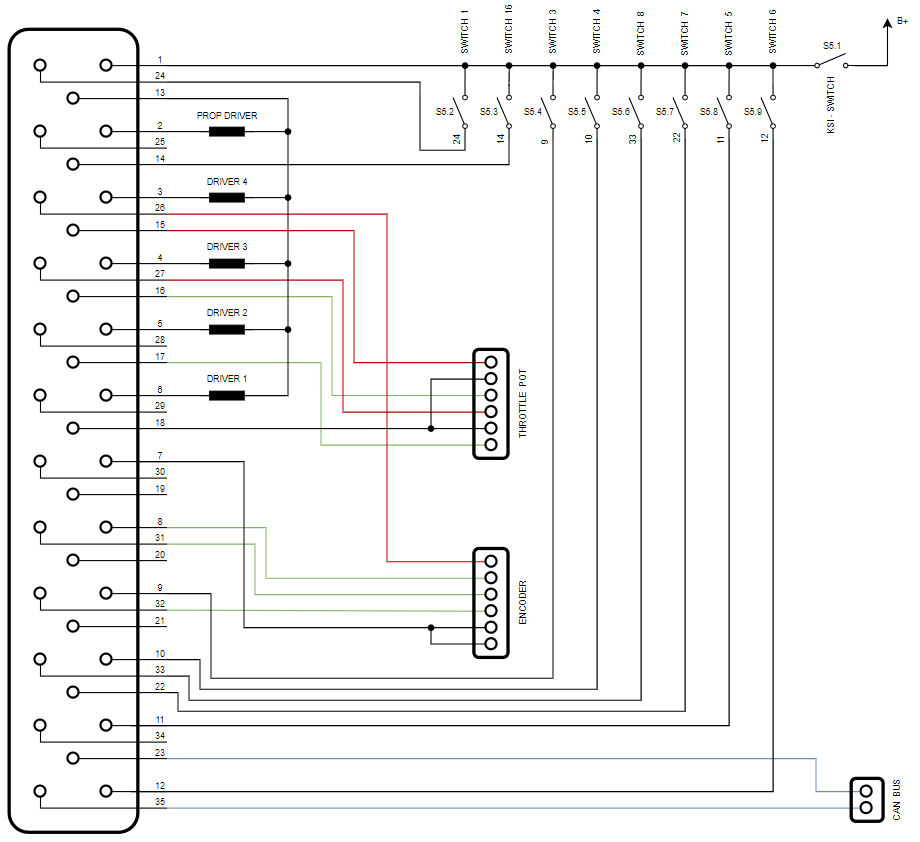
\includegraphics[scale=0.5]{figures/hcis/Antrieb_Steuerstromkreis.png}
		\caption{Grundaufbau des Steuerstromkreises}
	\end{center}
\end{figure}

\newpage



%% Digitale Eingänge (Digital Inputs) %%%%%%%%%%%%%%%%%%%%%%%%%%%%%%%%%%%%%%%%%%%%%%%
\subsubsection{Digitale Eingänge (Digital Inputs)}
Es gibt insgesamt 16 Pins, die als digitale Eingänge genutzt werden können, jedoch werden sieben Pins davon eigentlich als Ausgänge konfiguriert. 

\begin{figure}[H]
	\begin{center}
		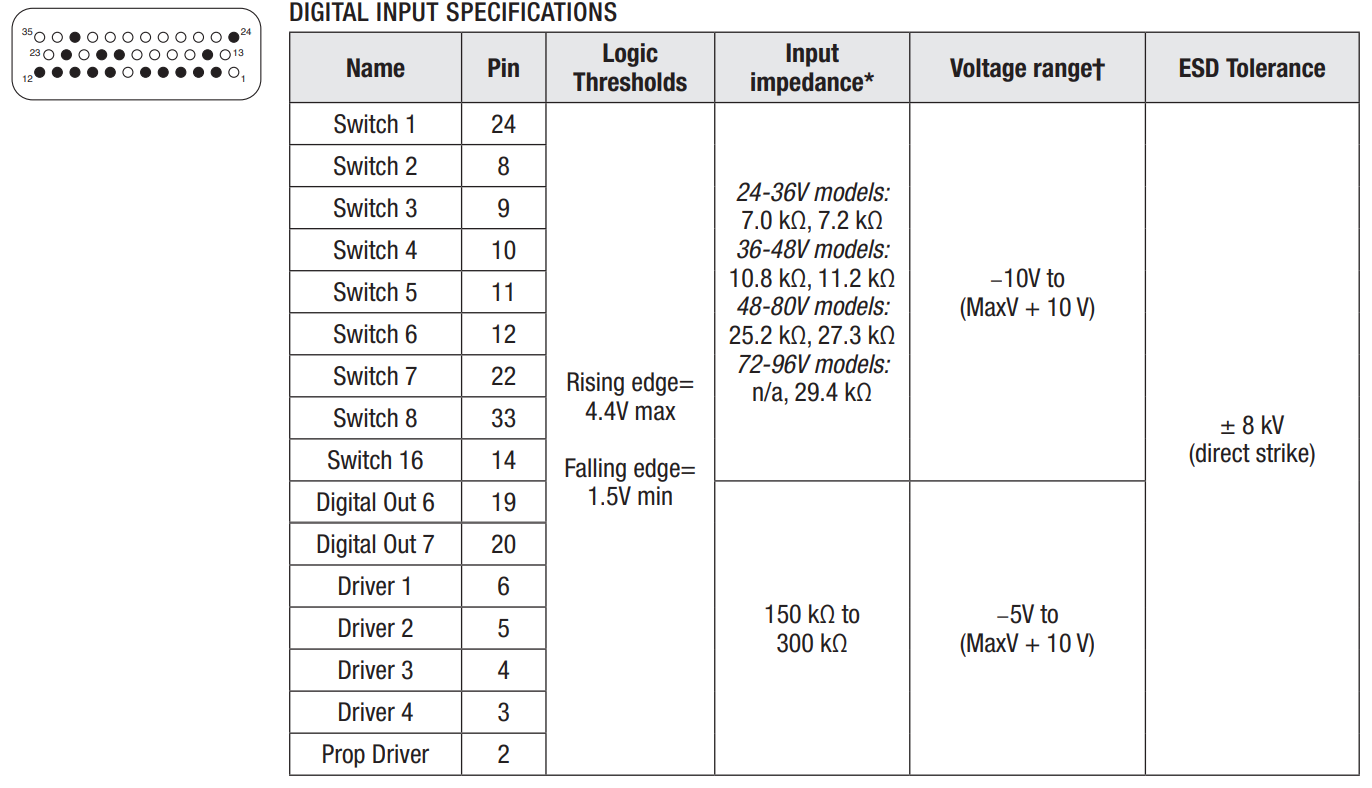
\includegraphics[width=\textwidth]{figures/hcis/Digital_Input_Specifications.png}
		\caption{Digital Input Specifications}
	\end{center}
\end{figure}




%% Analoge Eingänge (Analog Inputs) %%%%%%%%%%%%%%%%%%%%%%%%%%%%%%%%%%%%%%%%%%%%%%%
\subsubsection{Analoge Eingänge (Analog Inputs)}
Es gibt insgesamt zwei Pins die als analoge Eingänge verwendet werden können. Ein Pin davon wird jedoch im Normalfall für den Motortemperatur-Sensor verwendet. Die Eingänge, die für das Gas- und Bremspotentiometer verwendet werden, sind in dieser Kategorie nicht aufgelistet, obwohl diese ebenfalls als analoge Eingänge genutzt werden. Diese Pins sind jedoch speziell für die Gas- und Bremssteuerung konfiguriert und sollten im Normalfall auch dafür hergenommen werden.

\begin{figure}[H]
	\begin{center}
		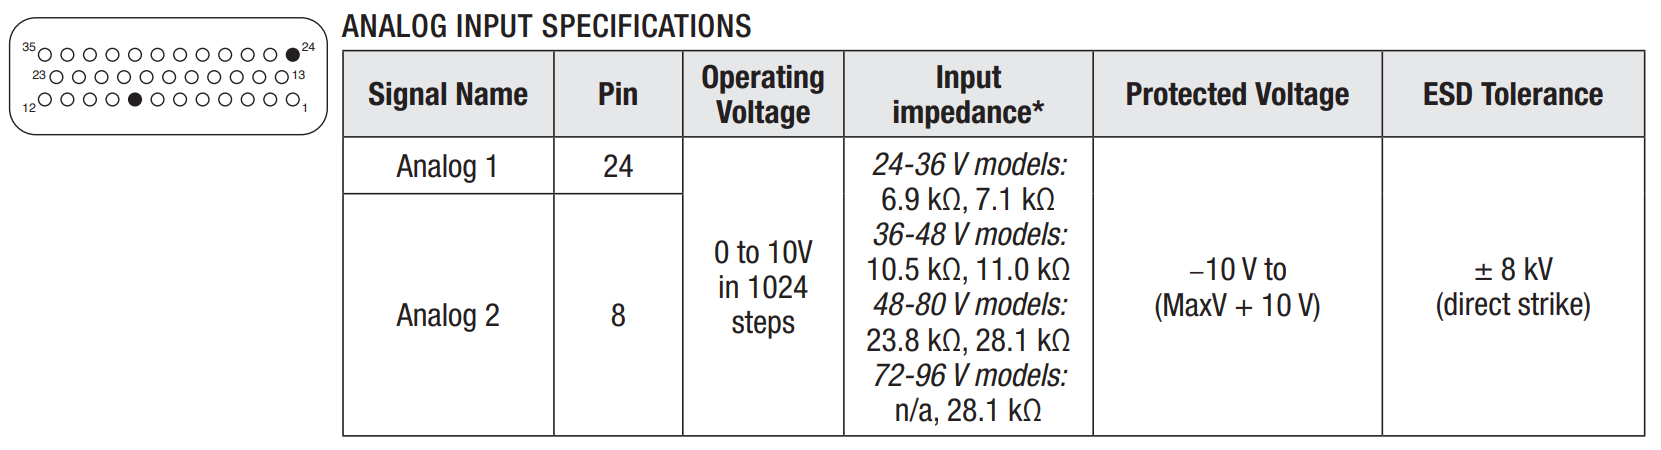
\includegraphics[width=\textwidth]{figures/hcis/Analog_Input_Specifications.png}
		\caption{Analog Input Specifications}
	\end{center}
\end{figure}



\newpage



%% Gas- und Bremseingänge (Throttle and Brake Inputs) %%%%%%%%%%%%%%%%%%%%%%%%%%%%%%%%%%%%%%%%%%%%%%%
\subsubsection{Gas- und Bremseingänge (Throttle and Brake Inputs)}
Die zwei Gas- oder Bremssteuerungs-Eingänge können unabhängig von einander programmiert werden. Sie sind optimiert für die Anwendung mittels Spannungssteuerung, 2-Draht Widerstandssteuerung oder 3-Draht Widerstandssteuerung. Bei der Spannungssteuerung benötigt man die Pins Pot Wiper und I/O Ground, bei der 2-Draht Widerstandssteuerung Pot Wiper und Pot Low und bei der 3-Draht Widerstandssteuerung Pot High, Pot Wiper und Pot Low. In unserem Fall benutzen wir beide Steuerungs-Eingänge für die 3-Draht Widerstandssteuerung, da der Gasdrehgriff über eine Drahtbrucherkennung verfügt. Das heißt, der Gasdrehgriff hat insgesamt zwei unabhängige 3-Draht Potentiometer-Ausgänge, welche beide für den Gaseingang benutzt werden.

\begin{figure}[H]
	\begin{center}
		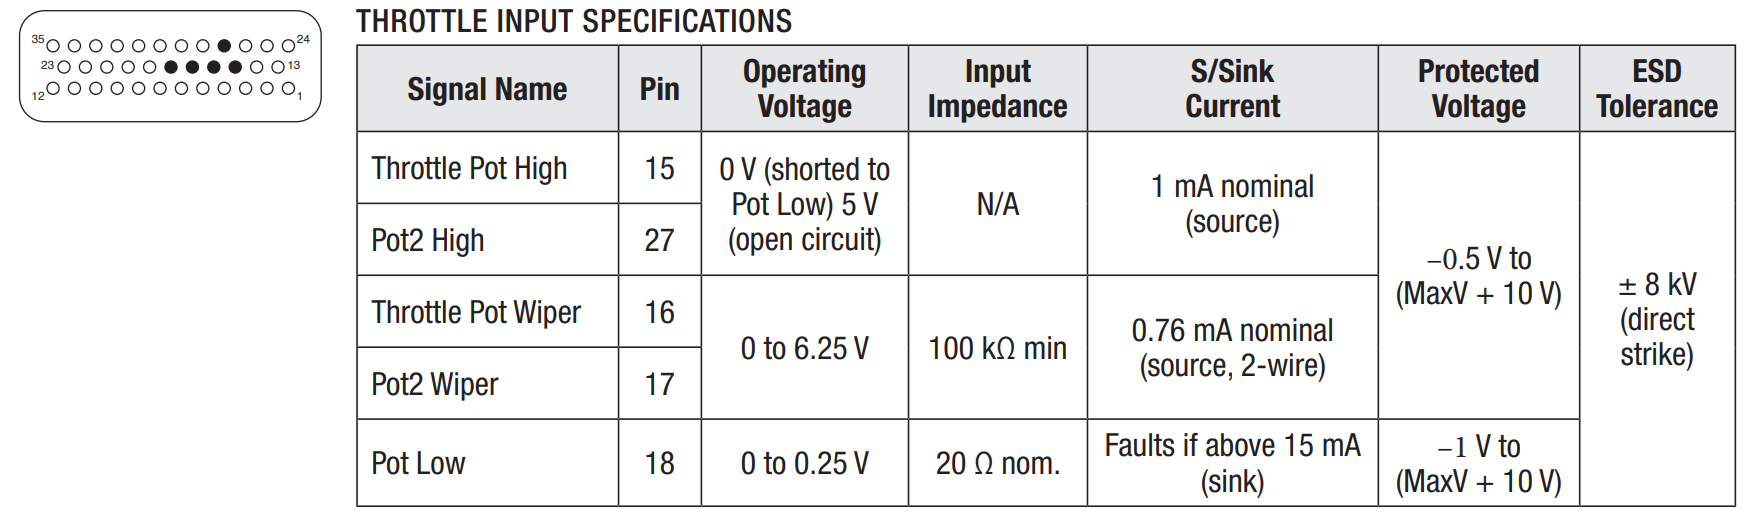
\includegraphics[width=\textwidth]{figures/hcis/Throttle_Input_Specifications.png}
		\caption{Throttle Input Specifications}
	\end{center}
\end{figure}



%% Positionsrückmeldung vom Encoder (Position-feedback Input) %%%%%%%%%%%%%%%%%%%%%%%%%%%%%%%%%%%%%%%%%%
\subsubsection{Positionsrückmeldung vom Encoder (Position-feedback Input)}
Diese zwei Pins sind intern dafür konfiguriert, die aktuelle Position der Motorwelle einzulesen, um eine optimale feldorienterte Ansteuerung des Motors durchführen zu können. Dabei gibt es die Möglichkeiten über einen Quadratur-Encoder oder einen Sin/Cos-Encoder. Da in dem Ashwoods-Motor ein Sin/Cos-Sensor verbaut ist, wurde dies vorab bei dem Motorcontroller eingestellt.

\begin{figure}[H]
	\begin{center}
		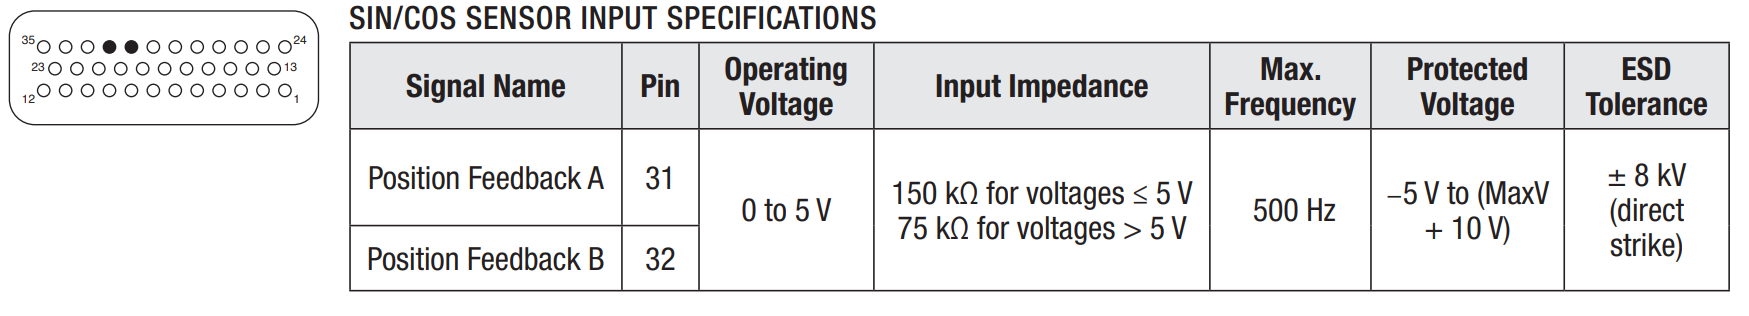
\includegraphics[width=\textwidth]{figures/hcis/SinCosSensor_Input_Specifications.png}
		\caption{Sin/Cos Sensor Input Specifications}
	\end{center}
\end{figure}


\newpage


%% Prozessorversorgung und Spulenrücklauf (KSI and Coil Return) %%%%%%%%%%%%%%%%%%%%%%%%%%%%%%%%%%%%%%
\subsubsection{Prozessorversorgung und Spulenrücklauf (KSI and Coil Return)}
Der KSI-Eingang stellt die elektrische Versorgung aller Niederleistungs-Schaltkreise zur Verfügung. Dies  beinhaltet ebenfalls die Versorgung aller Ausgänge und die Kondensator-Vorlade-Funktion, welche dazu dient, die Kondensatoren vorzuladen, um hohe Einschaltströme zu verhindern. Der Spulenrücklauf ist speziell für den Rücklauf der pulsweitenmodulierbaren Ausgänge konfiguriert worden, um ein übrmäßiges Schaltrauschen zu verhindern.

\begin{figure}[H]
	\begin{center}
		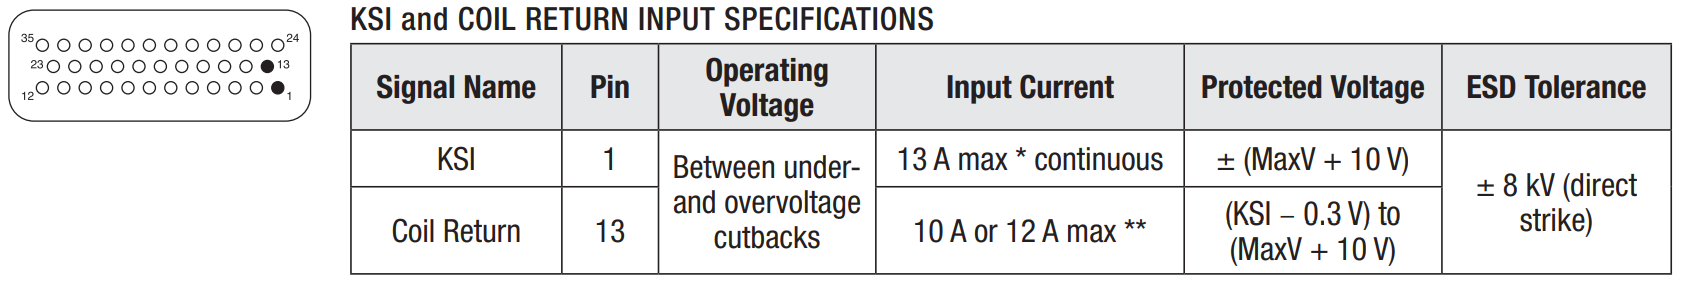
\includegraphics[width=\textwidth]{figures/hcis/KSI_CoilReturn_Input_Specifications.png}
		\caption{KSI and Coil Return Input Specifications}
	\end{center}
\end{figure}



%% Analoge Ausgänge (Analog Outputs %%%%%%%%%%%%%%%%%%%%%%%%%%%%%%%%%%%%%%%%%%%%%%%
\subsubsection{Analoge Ausgänge (Analog Outputs)}
Der analoge Ausgang kann ein Spannungssignal von 0 bis 10V ausgeben. Dieser Ausgang ist für die Ausgabe über Anzeigeinstrumente, wie zum Beispiel eine Anzeige über den aktuellen Ladestand des Akkumulators, vorgesehen.

\begin{figure}[H]
	\begin{center}
		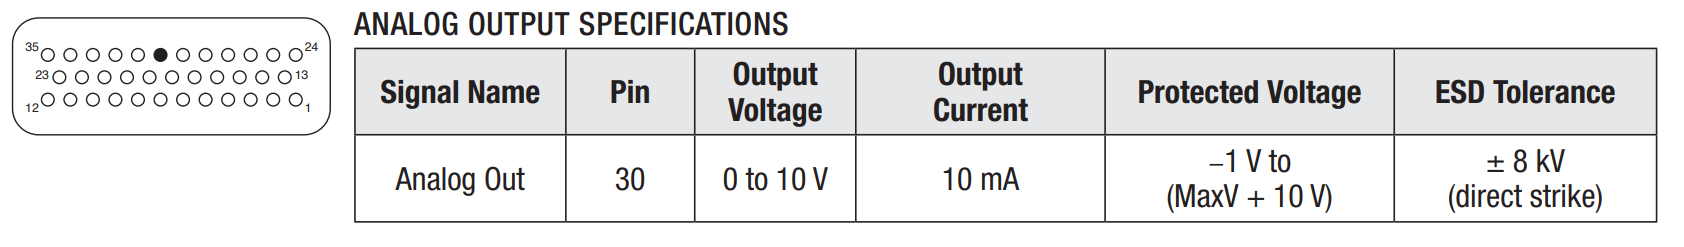
\includegraphics[width=\textwidth]{figures/hcis/Analog_Output_Specifications.png}
		\caption{Analog Output Specifications}
	\end{center}
\end{figure}


\newpage



%% Digitale und Pulsweitenmodulierbare Ausgänge (Digital and PWM Outputs) %%%%%%%%%%%%%%%%%%%%%%%%%%%%
\subsubsection{Digitale und Pulsweitenmodulierbare Ausgänge (Digital and PWM Outputs)}
Es gibt insgesamt 7 digitale Ausgänge, wovon jedoch nur 5 für eine Pulsweitenmodulation konfiguriert werden können. Diese Ausgänge sind für induktive Lasten, wie zum Beispiel den Hauptschütz oder eine elektromagnetische Bremse, vorgesehen. Rein ohmsche Lasten können ebenfalls gesteuert werden, jedoch darf der zulässige Spitzenstrom nicht überschritten werden. Der Proportional-Driver kann bei richtiger Konfiguration auch für die Anzeige eines Tachometers hergenommen werden. Diese Gruppe kann ebenfalls als digitaler Eingang benutzt werden.

\begin{figure}[H]
	\begin{center}
		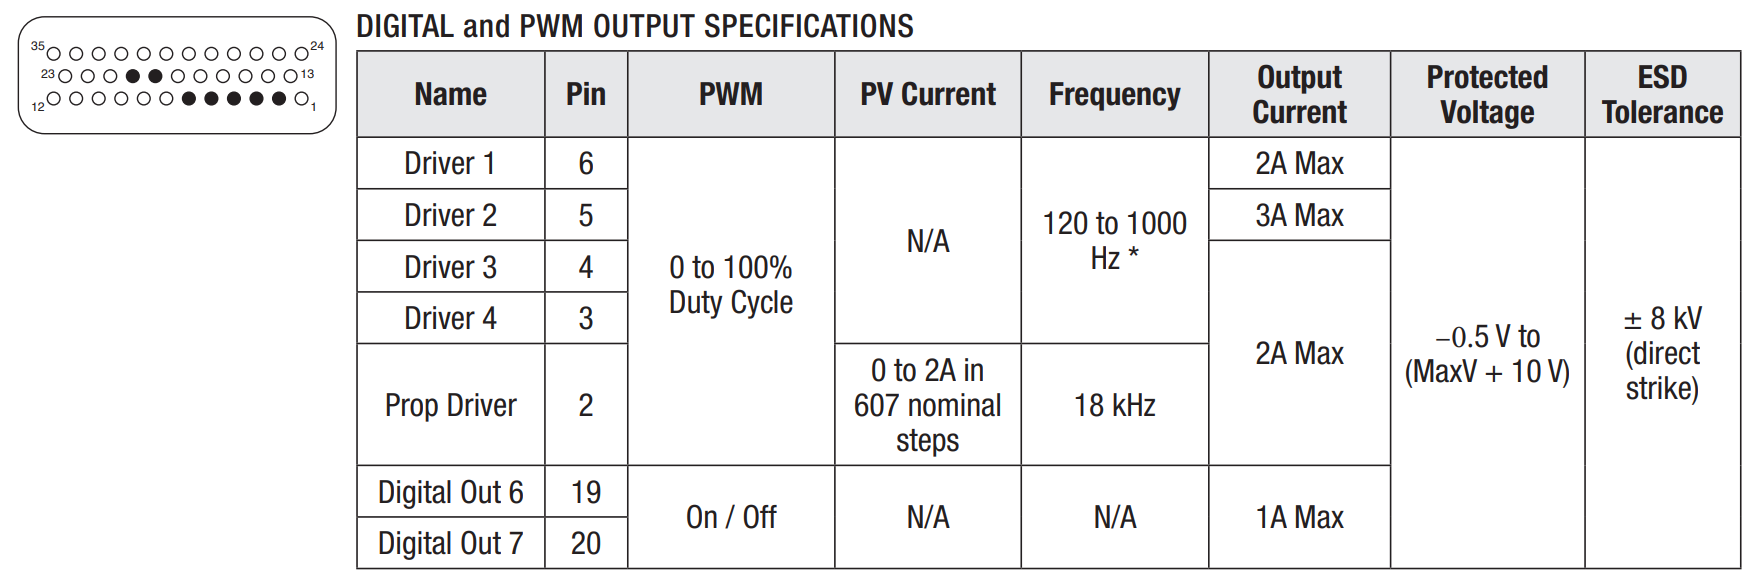
\includegraphics[width=\textwidth]{figures/hcis/Digital_PWM_Output_Specifications.png}
		\caption{Digital and PWM Output Specifications}
	\end{center}
\end{figure}



%% Spannungsversorgungs-Ausgänge (Power Supply Outputs) %%%%%%%%%%%%%%%%%%%%%%%%%%%%%%%%%%%%%%%%%%%%%%
\subsubsection{Spannungsversorgungs-Ausgänge (Power Supply Outputs)}
Um kleine Schaltkreise, wie zum Beispiel einen LED-Indikator oder die Positionsrückmeldung vom Encoder, mit Spannung versorgen zu können, gibt es zwei dafür vorgesehene Spannungsversorgungs-Ausgänge mit einem Pin für 5V und 12V. Für diese Anwendungen gibt es ebenfalls noch einen Rücklauf, der als I/O Ground definiert wurde.

\begin{figure}[H]
	\begin{center}
		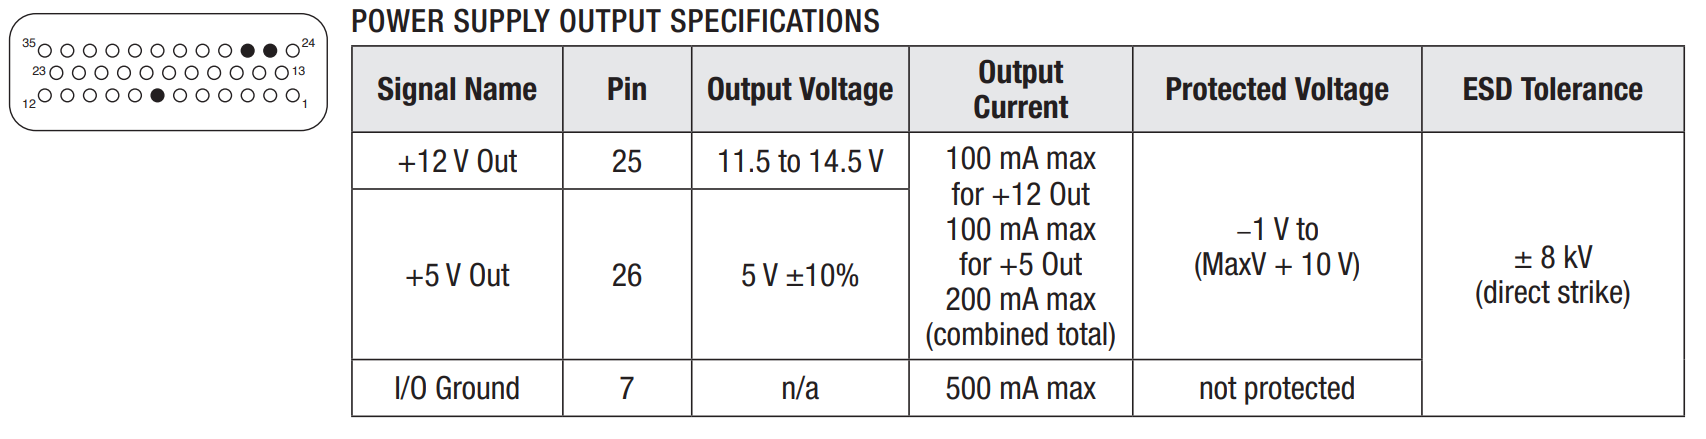
\includegraphics[width=\textwidth]{figures/hcis/Power_Supply_Output_Specifications.png}
		\caption{Power Supply Output Specifications}
	\end{center}
\end{figure}


\newpage


%% Kommunikations-Ports %%%%%%%%%%%%%%%%%%%%%%%%%%%%%%%%%%%%%%%%%%%%%%%
\subsubsection{Kommunikations-Ports}
Für die Kommunikation mit anderen Betriebsmitteln stellt uns der Motorcontroller zwei Möglichkeiten zur Verfügung, den CAN-Bus und die serielle Schnittstelle. Da sich unser Projektteam auf die Nutzung des CAN-Buses geeinigt hat, wird die serielle Schnittstelle nicht verwendet. Die zwei Pins CAN Term High und CAN Term Low werden ebenfalls nicht benötigt, denn diese dienen nur dazu, den CAN-Bus vorübergehend funktionsunfähig zu schalten. Programmtechnisch gibt es drei Möglichkeiten vom Motorcontroller zur Konfiguration des CAN-Buses, dies wird jedoch im Punkt Software genauer erklärt.

\begin{figure}[H]
	\begin{center}
		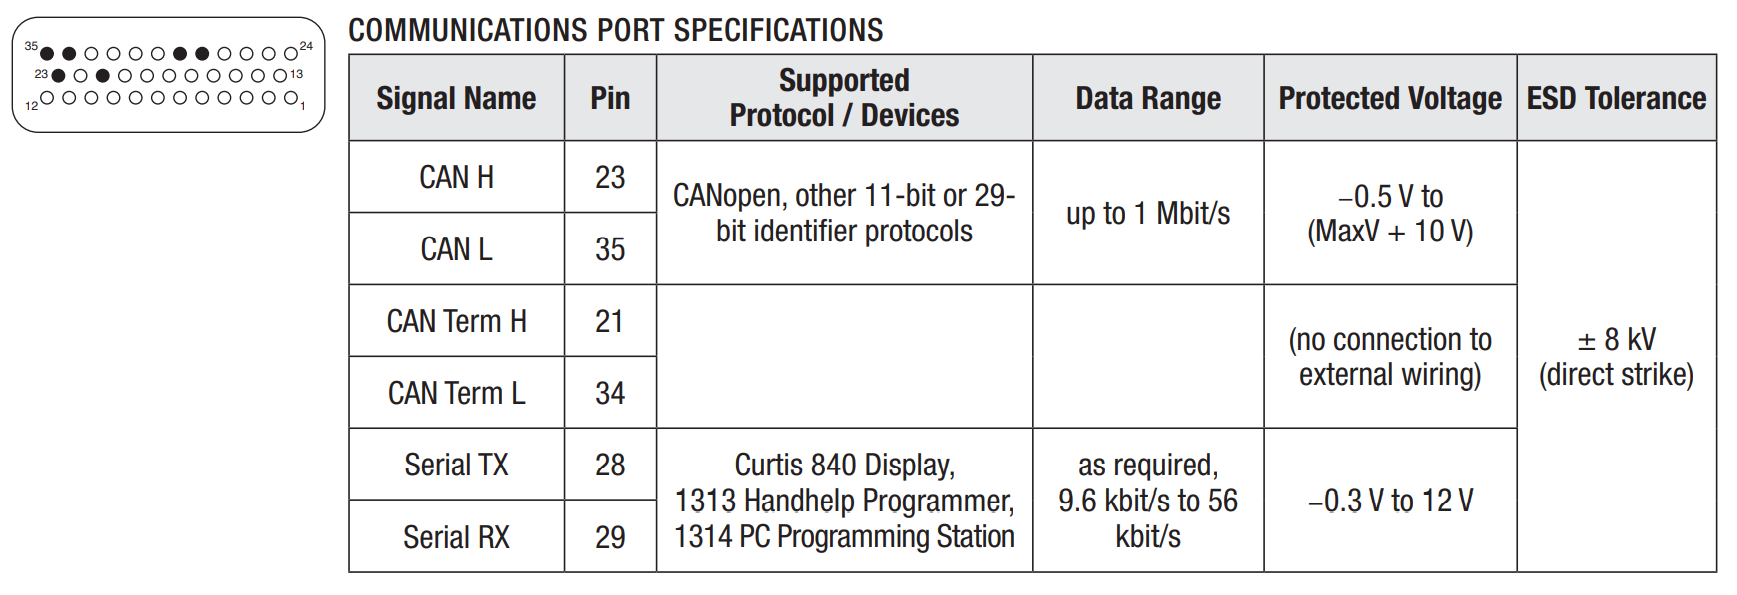
\includegraphics[width=\textwidth]{figures/hcis/Communications_Port_Specifications.png}
		\caption{Communications Port Specifications}
	\end{center}
\end{figure}



\newpage



%% Softwareaufbau %%%%%%%%%%%%%%%%%%%%%%%%%%%%%%%%%%%%%%%
\section{Softwareaufbau des Antriebssystems}


%% Steuerung der In- und Outputs %%%%%%%%%%%%%%%%%%%%%%%%%%%%%%%%%%%%%%%%%%%%
\section{ Steuerung der Ein- und Ausgänge (I/O Assingment)}
\subsection{Funktionen}
\subsection{Zuweisung}


%% Drehmomentsteuerung %%%%%%%%%%%%%%%%%%%%%%%%%%%%%%%%%%%%%%%%%%%%
\section{Drehmomentsteuerung (Torquecontrol)}
\subsection{Grundfunktion}
\subsection{Parameter}


%% Kommunikation %%%%%%%%%%%%%%%%%%%%%%%%%%%%%%%%%%%%%%%%
\section{Kommunikation (CAN-Bus)}
\subsection{Grundfunktion}
\subsubsection{Parameter}
